\documentclass[11pt,a4paper]{article}

% These are extra packages that you might need for writing the equations:
\usepackage{amsmath}
\usepackage{amsfonts}
\usepackage{amssymb}
\usepackage{booktabs}
\usepackage{hyperref}
\usepackage{listings}
\usepackage{xcolor}
\usepackage{outlines}
\usepackage{mathtools}

\lstset {language=C++,
		 basicstyle=\ttfamily,
         keywordstyle=\color{blue}\ttfamily,
         stringstyle=\color{red}\ttfamily,
         commentstyle=\color{purple}\ttfamily,
         morecomment=[l][\color{magenta}]{\#},
       	 basicstyle=\tiny}

% You need the following package in order to include figures in your report:
\usepackage{graphicx}

% With this package you can set the size of the margins manually:
\usepackage[left=2cm,right=2cm,top=2cm,bottom=2cm]{geometry}


\begin{document}

% Enter the exercise number, your name and date here:
\noindent\parbox{\linewidth}{
 \parbox{.25\linewidth}{ \large ICP, Exercise 10 }\hfill
 \parbox{.5\linewidth}{\begin{center} \large Beat Hubmann \end{center}}\hfill
 \parbox{.2\linewidth}{\begin{flushright} \large Dec 03, 2018 \end{flushright}}
}
\noindent\rule{\linewidth}{2pt}


\section{Introduction}

An explicit Runge-Kutta method was implemented to solve the equation of motion
for an inclined throw with air resistance in two dimensions.

\section{Algorithm Description}
The Runge-Kutta family of methods to solve ordinary differential equations is well known and described.
The algorithm implemented is the classical and most used Runge-Kutta method usually referred to as RK4 or
something closely similar.

\section{Results}

The program was implemented as described above and submitted with this report. 

\subsection{Task 1}
For a fixed friction coefficient $\gamma = 1.0$, trajectories were calculated for launch velocities $v \in \{5, 10, 20, 40\}\ \text{m/s}$ and 
over a range of launch angles $10 \le \alpha \le 80\ \text{deg}$ over 15'000 time steps of size
$\Delta t = 0.001\ \text{s}$. The results are shown in figures~\ref{fig:1_1}, \ref{fig:1_2},
\ref{fig:1_3} and~\ref{fig:1_4}.

\begin{figure}[ht]
\begin{center}
\includegraphics[scale=1.2]{figure1_1.eps} 
\end{center}
\caption{Flight trajectories for $\gamma = 1.0$, $v= 5.0$.}
\label{fig:1_1}
\end{figure}

\begin{figure}[ht]
\begin{center}
\includegraphics[scale=1.2]{figure1_2.eps} 
\end{center}
\caption{Flight trajectories for $\gamma = 1.0$, $v= 10.0$.}
\label{fig:1_2}
\end{figure}

\begin{figure}[ht]
\begin{center}
\includegraphics[scale=1.2]{figure1_3.eps} 
\end{center}
\caption{Flight trajectories for $\gamma = 1.0$, $v= 20.0$.}
\label{fig:1_3}
\end{figure}

\begin{figure}[ht]
\begin{center}
\includegraphics[scale=1.2]{figure1_4.eps} 
\end{center}
\caption{Flight trajectories for $\gamma = 1.0$, $v= 40.0$.}
\label{fig:1_4}
\end{figure}

\subsection{Task 2}
For a fixed launch velocity $v = 40.0\ \text{m/s}$, the friction coefficient was varied such
that $0.25 \le \gamma \le 10.0$ and the maximum obtained flight distance $x$ recorded.
The result is shown in figure~\ref{fig:2}.

\begin{figure}[ht]
    \begin{center}
    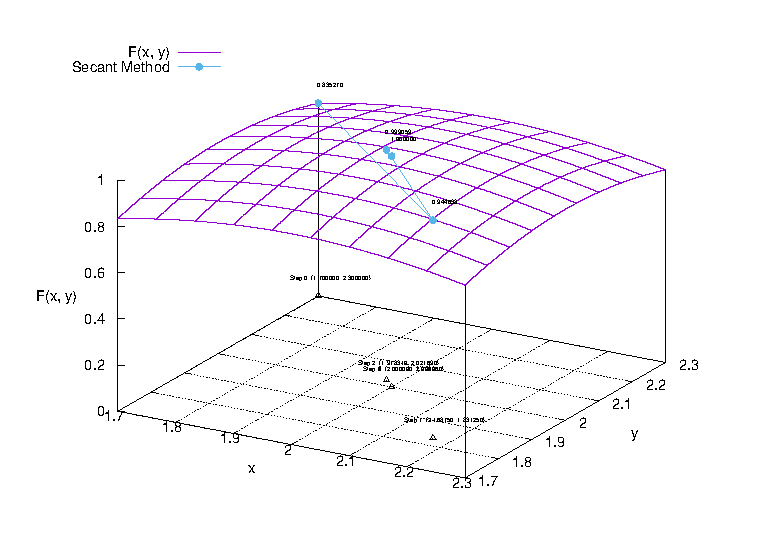
\includegraphics[scale=1.2]{figure2.eps} 
    \end{center}
    \caption{Launch angle $a_{max}$ for maximum range as function of friction coeffcient $\gamma$, $v= 40.0$.}
    \label{fig:2}
\end{figure}
    
\section{Discussion}
The results seem physically plausible. No error analysis was performed.\\
Considerable effort went into templating the solver for generic use for the 
purpose of practice following the example of~\cite{Gottschling}.

\begin{thebibliography}{99}


% \bibitem{metropolis}
% Metropolis, N.,
% Rosenbluth, A.W.,
% Rosenbluth, M.N.,
% Teller, A.H.,
% Teller, E.\\
% \emph{Equations of State Calculations by Fast Computing Machines},\\
% Journal of Chemical Physics. 21 (6): 1087,\\
% 1953.


% \bibitem{herrmann}
% 	Herrmann, H. J.,
% 	Singer, H. M.,
% 	Mueller L.,
% 	Buchmann, M.-A.,\\
% 	\emph{Introduction to Computational Physics - Lecture Notes},\\
% 	ETH Zurich,\\
% 	2017.

\bibitem{Gottschling}
Gottschling, Peter\\
\emph{Discovering Modern C++},\\
Addison-Wesley,\\
2016.




\end{thebibliography}

\end{document}